\section{Sécurité}

\begin{frame}{Sécurité}  
\end{frame}

\begin{frame}{Enjeux de la sécurité}

  \begin{block}{Tout est une question de \underline{risques}}
    Risque = un impact x probabilité d'occurrence
  \end{block}

  \begin{block}{Rédaction d'un modèle de menaces (\textit{threats modelling})}
    Quatre questions à se poser\footnote{\url{https://owasp.org/www-community/Threat_Modeling}}:
    \begin{itemize}
    \item Sur quoi travaillons-nous ?
    \item Qu'est-ce qu'il pourrait arriver de mauvais ?
    \item Quoi faire si cela arrive ?
    \item Avons-nous fait du bon travail ?
    \end{itemize}
  \end{block}
\end{frame}

\begin{frame}{OWASP}
  \begin{block}{Top 10}
    \begin{itemize}
    \item \textit{Open Web Application Security Project}.
    \item Propose (entre autres) un classement des 10 risques de
      sécurités les plus critiques.
    \end{itemize}
  \end{block}
\end{frame}

\begin{frame}{OWASP 2021}
  \begin{block}{Le top 10 des menaces de sécurité}
    Version 2021 du Top 10 OWASP\footnote{\url{https://owasp.org/Top10/fr/}}:
    \begin{enumerate}
    \item Contrôles d'accès défaillants.
    \item Défaillances cryptographiques.
    \item Injections.
    \item Conception non-sécurisée.
    \item Mauvaise configuration de sécurité.
    \item Composants vulnérables et obsolètes.
    \item Identification et authentification de mauvaise qualité.
    \item Manque d'intégrité des données et du logiciel.
    \item Carence des systèmes de contrôle et de journalisation.
    \item Falisification des requêtes côté serveur.
    \end{enumerate}
  \end{block}
\end{frame}

\begin{frame}{Comparaison avec l'OWASP 2017}
  \begin{center}
    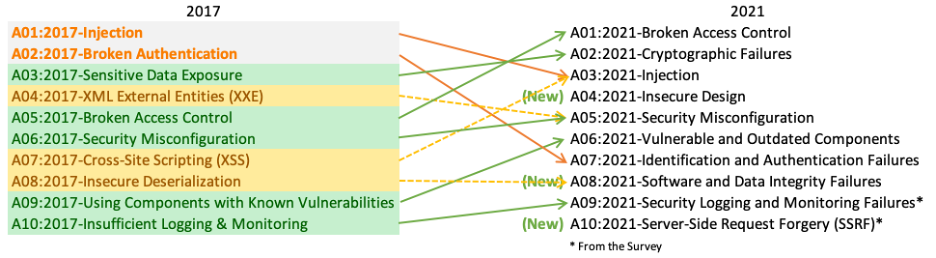
\includegraphics[scale=0.7]{images/owasp_mapping.png}
  \end{center}
\end{frame}

\begin{frame}{Sécurité mise en place par Django}
  \begin{block}{Protection contre les attaques XSS}
    Le système de \textit{template} de django échappe certains
    caractères \textbf{mais} ne protège pas contre toutes les
    attaques XSS\footnote{\url{https://docs.djangoproject.com/fr/4.1/topics/security/}}.
    \begin{itemize}
    \item \textit{via} du code HTML et JS dans les variables
    \item \textit{via} du code HTML en base de données
    \end{itemize}
  \end{block}

  \begin{block}{Protection contre les attaques CSRF}
    Protection par le \textit{middleware} \textsf{CSRFViewMiddleware}.
    Cependant il faut être prudent lors de l'utilisation du décorateur
    \textsf{csrf\_exempt}.
  \end{block}

  \begin{block}{Protection contre les injections SQL}
    À moins que l'on n'écrive des requêtes en SQL brutes, le système
    de paramétrisation apporte une protection aux injections SQL.
  \end{block}
\end{frame}

\begin{frame}{Sécurité et configuration de Django}
  \begin{block}{Autres protections\footnote{\url{https://docs.djangoproject.com/fr/4.1/topics/security/}}}
    \begin{itemize}
    \item Détournement de clic (\textit{via} les \textit{frames} HTML).
    \item SSL et HTTPS.
    \item Validation de l'entête HTTP ``Host''.
    \item Sécurité des sessions.
    \item ...
    \end{itemize}
  \end{block}

  \begin{block}{Mise en production}
    Django propose une commande permettant de vérifier la sécurité
    d'une application web avant sa mise en production.
    
    \textsf{./manage.py check --deploy}
  \end{block}
\end{frame}

\begin{frame}{Renforcer la sécurité}
  \begin{block}{Sécurités supplémentaires}
    \begin{itemize}
    \item Authentification par nom d'utilisateur et mot de passe:
      \begin{itemize}
      \item Vérification de la sécurité du mot de passe.
      \end{itemize}
    \item Mise en place d'un système de rôles:
      \begin{itemize}
      \item Administrateur
      \item Auteur d'un projet, d'un problème ou d'un commentaire
      \item Collaborateur
      \item Utilisateur
      \end{itemize}
    \end{itemize}
  \end{block}
\end{frame}

\begin{frame}{Tester la sécurité de l'API}
  \begin{block}{Différents types de tests}
    \begin{itemize}
    \item \textit{Scan} de vulnérabilités
    \item Tests de pénétrations
    \item Audits de sécurité
    \item ...
    \end{itemize}

    Comment tester la sécurité de l'API ?
  \end{block}

  \begin{block}{\textit{Via} Django}
    Il est possible d'utiliser les tests Django pour vérifier la
    sécurité du système développé. Il existe différents niveaux de
    tests: ici nous parlons de tests non fonctionnels d'acceptations
    et non pas de tests fonctionnels unitaires ($\rightarrow$ en
    complément, non pas à la place).
  \end{block}
\end{frame}


\begin{frame}{Respect de la RGPD}
  \begin{block}{Quelques points importants pour le respect de la RGPD}
    \begin{itemize}
    \item Les données personnelles sont chiffrées dans la base de données.
    \item Un utilisateur connecté peut actualiser ou supprimer toutes
      les ressources dont il est l'auteur.
    \item Les données personnelles stockées en base de données sont réduites.
    \item Après publication, il doit être possible pour un utilisateur de
      demander la suppression de toutes ses données personnelles.
    \item $\rightarrow$ C'est une question de droit, la consultation
      d'un juriste est souvent conseillée.
    \end{itemize}

    $\rightarrow$ Voir \url{https://www.economie.gouv.fr/entreprises/reglement-general-sur-protection-des-donnees-rgpd}
  \end{block}
\end{frame}

